%
%\begin{tikzpicture}
%
%% Axes
%\draw[thick,->] (0,0)--(0,6.5) node[above]{$z$};
%\draw[thick,->] (0,0) node[left]{$0$} --(7,0) node[right]{$n$};
%
%% hire fire
%\draw[blue,dotted] (0,0) ..controls (2,2.5) and (4,4.5) .. (6.5,4.5);
%\draw[blue,dotted] (2.05,2.32)..controls (2.35,2.5) and (4,4.5) .. (6.5,4.5) ;
%\draw[blue,thick] (2.35,2.6)..controls (2.35,2.5) and (4,4.5) .. (6.5,4.5) node[right]{Hire / Fire};
%%node[above,yshift=-1pt]{Hire} node[below,yshift=-1pt]{Fire};
%
%% stay exit
%\draw[blue,thick] (0.5,6) ..controls (0.55,5) and (0.75,3) .. (1.33,2.6);
%\draw[blue,thick] (1.33,2.6) ..controls (4,2.6) ..  (7,2.6) node[right]{Stay / Exit} ;
%\draw[blue,dotted] (0.5,6) ..controls (0.75,2.5) and (1.25,2) .. (3,2.5);
%\draw[blue,dotted] (3,2.5) ..controls (4,2.75) and (5,3.15) .. (6.5,3.4);
%%node[above,yshift=-1pt]{Stay} node[below,yshift=-1pt]{Exit};
%
%
%% dn = 0
%\draw[black,dotted](0,0) ..controls (0.5, 1.3) and (1,2) ..(1.3,2.6) ;
%\draw[black,thick] (1.3,2.6) ..controls (2,4) and (3,5.5) .. (4.3,6) node[above, yshift=2pt]{$dn=0$};
%
%
%% Regions
%\draw (4.75,3.45) node{\alert{\textbf{Stay \& Fire}}};
%\draw (4,0.5) node{\alert{\textbf{Exit}}};
%\draw (2.2,6) node{\alert{\textbf{Hire \& Grow}}};
%\draw (4.6,5.1) node{\alert{\textbf{Hire \& Shrink}}};
%
%
%\end{tikzpicture}




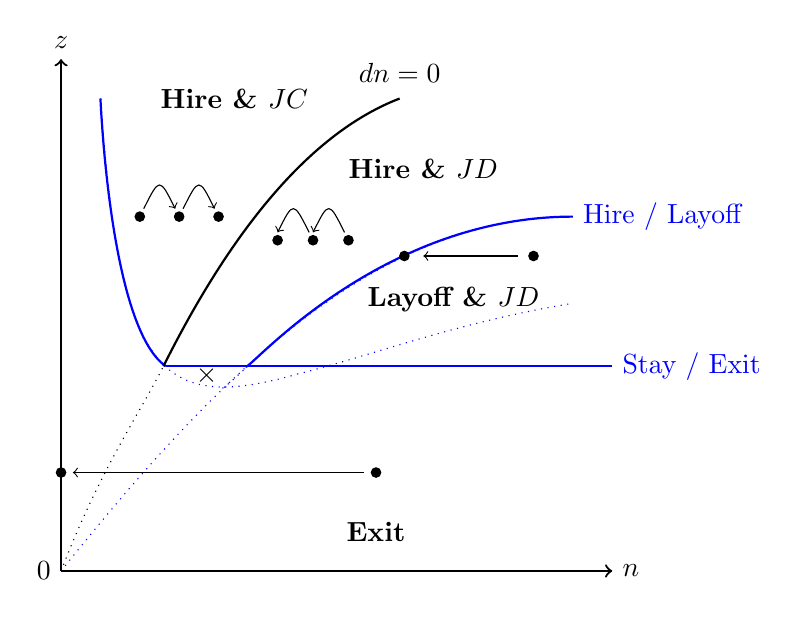
\begin{tikzpicture}

% Axes
\draw[thick,->] (0,0)--(0,6.5) node[above]{$z$};
\draw[thick,->] (0,0) node[left]{$0$} --(7,0) node[right]{$n$};

% hire fire
\draw[blue,dotted] (0,0) ..controls (2,2.5) and (4,4.5) .. (6.5,4.5);
\draw[blue,dotted] (2.05,2.32)..controls (2.35,2.5) and (4,4.5) .. (6.5,4.5) ;
\draw[blue,thick] (2.35,2.6)..controls (2.35,2.5) and (4,4.5) .. (6.5,4.5) node[right]{Hire / Layoff};
%node[above,yshift=-1pt]{Hire} node[below,yshift=-1pt]{Fire};

% stay exit
\draw[blue,thick] (0.5,6) ..controls (0.55,5) and (0.75,3) .. (1.33,2.6);
\draw[blue,thick] (1.33,2.6) ..controls (4,2.6) ..  (7,2.6) node[right]{Stay / Exit} ;
\draw[blue,dotted] (0.5,6) ..controls (0.75,2.5) and (1.25,2) .. (3,2.5);
\draw[blue,dotted] (3,2.5) ..controls (4,2.75) and (5,3.15) .. (6.5,3.4);
%node[above,yshift=-1pt]{Stay} node[below,yshift=-1pt]{Exit};


% dn = 0
\draw[black,dotted](0,0) ..controls (0.5, 1.3) and (1,2) ..(1.3,2.6) ;
\draw[black,thick] (1.3,2.6) ..controls (2,4) and (3,5.5) .. (4.3,6) node[above, yshift=2pt]{$dn=0$};


% Regions
\draw (4.75,3.45) node{\alert{\textbf{$\:\:\:\:\:\:$Layoff \& $JD$}}};
\draw (4,0.5) node{\alert{\textbf{Exit}}};
\draw (2.2,6) node{\alert{\textbf{Hire \& $JC$}}};
\draw (4.6,5.1) node{\alert{\textbf{Hire \& $JD$}}};


% Actions

% exit
\draw[fill] (4,1.25) circle [radius=0.06];
\draw[->] (3.85,1.25)--(0.15,1.25);
\draw[fill] (0,1.25) circle [radius=0.06];

% fire and stay
\draw[fill] (6,4) circle [radius=0.06];
\draw[->] (5.8,4)--(4.6,4);
\draw[fill] (4.36,4) circle [radius=0.06];


% hire and grow
\draw[fill] (1,4.5) circle [radius=0.06];
\draw[->] (1.05,4.6)..controls (1.25,5) ..(1.45,4.6);
\draw[fill] (1.5,4.5) circle [radius=0.06];
\draw[->] (1.55,4.6)..controls (1.75,5) ..(1.95,4.6);
\draw[fill] (2,4.5) circle [radius=0.06];


% shire and hrink
\draw[fill] (3.65,4.2) circle [radius=0.06];
\draw[->] (3.6,4.3)..controls (3.4,4.7) ..(3.2,4.3);
\draw[fill] (3.2,4.2) circle [radius=0.06];
\draw[->] (3.15,4.3)..controls (2.95,4.7) ..(2.75,4.3);
\draw[fill] (2.75,4.2) circle [radius=0.06];

\draw (1.85,2.48) node{\alert{\textbf{$\times$}}};

\end{tikzpicture}
